%%%%%%%%%%%%%%
%% Run LaTeX on this file several times to get Table of Contents,
%% cross-references, and citations.

%% If you have font problems, you may edit the w-bookps.sty file
%% to customize the font names to match those on your system.

%% w-bksamp.tex. Current Version: Feb 16, 2012
%%%%%%%%%%%%%%%%%%%%%%%%%%%%%%%%%%%%%%%%%%%%%%%%%%%%%%%%%%%%%%%%
%
%  Sample file for
%  Wiley Book Style, Design No.: SD 001B, 7x10
%  Wiley Book Style, Design No.: SD 004B, 6x9
%
%
%  Prepared by Amy Hendrickson, TeXnology Inc.
%  http://www.texnology.com
%%%%%%%%%%%%%%%%%%%%%%%%%%%%%%%%%%%%%%%%%%%%%%%%%%%%%%%%%%%%%%%%

%%%%%%%%%%%%%
% 7x10
%\documentclass{wileySev}

% 6x9
\documentclass{wileySix}

\usepackage{graphicx}

%%%%%%%
%% for times math: However, this package disables bold math (!)
%% \mathbf{x} will still work, but you will not have bold math
%% in section heads or chapter titles. If you don't use math
%% in those environments, mathptmx might be a good choice.

% \usepackage{mathptmx}

% For PostScript text
\usepackage{w-bookps}

%%%%%%%%%%%%%%%%%%%%%%%%%%%%%%%%%%%%%%%%%%%%%%%%%%%%%%%%%%%%%%%%
%% Other packages you might want to use:

% for chapter bibliography made with BibTeX
% \usepackage{chapterbib}

% for multiple indices
% \usepackage{multind}

% for answers to problems
% \usepackage{answers}

%%%%%%%%%%%%%%%%%%%%%%%%%%%%%%
%% Change options here if you want:
%%
%% How many levels of section head would you like numbered?
%% 0= no section numbers, 1= section, 2= subsection, 3= subsubsection
%%==>>
\setcounter{secnumdepth}{3}

%% How many levels of section head would you like to appear in the
%% Table of Contents?
%% 0= chapter titles, 1= section titles, 2= subsection titles, 
%% 3= subsubsection titles.
%%==>>
\setcounter{tocdepth}{2}

%% Cropmarks? good for final page makeup
%% \docropmarks

%%%%%%%%%%%%%%%%%%%%%%%%%%%%%%
%
% DRAFT
%
% Uncomment to get double spacing between lines, current date and time
% printed at bottom of page.
% \draft
% (If you want to keep tables from becoming double spaced also uncomment
% this):
% \renewcommand{\arraystretch}{0.6}
%%%%%%%%%%%%%%%%%%%%%%%%%%%%%%

%%%%%%% Demo of section head containing sample macro:
%% To get a macro to expand correctly in a section head, with upper and
%% lower case math, put the definition and set the box 
%% before \begin{document}, so that when it appears in the 
%% table of contents it will also work:

\newcommand{\VT}[1]{\ensuremath{{V_{T#1}}}}

%% use a box to expand the macro before we put it into the section head:

\newbox\sectsavebox
\setbox\sectsavebox=\hbox{\boldmath\VT{xyz}}

%%%%%%%%%%%%%%%%% End Demo


\begin{document}


\booktitle{Survey Methodology}
\subtitle{This is the Subtitle}

\authors{Robert M. Groves\\
\affil{Universitat de les Illes Balears}
Floyd J. Fowler, Jr.\\
\affil{University of New Mexico}
}

\offprintinfo{Survey Methodology, Second Edition}{Robert M. Groves}

%% Can use \\ if title, and edition are too wide, ie,
%% \offprintinfo{Survey Methodology,\\ Second Edition}{Robert M. Groves}

%%%%%%%%%%%%%%%%%%%%%%%%%%%%%%
%% 
\halftitlepage

\titlepage


\begin{copyrightpage}{2007}
Survey Methodology / Robert M. Groves . . . [et al.].
\       p. cm.---(Wiley series in survey methodology)
\    ``Wiley-Interscience."
\    Includes bibliographical references and index.
\    ISBN 0-471-48348-6 (pbk.)
\    1. Surveys---Methodology.  2. Social 
\  sciences---Research---Statistical methods.  I. Groves, Robert M.  II. %
Series.\\

HA31.2.S873 2007
001.4'33---dc22                                             2004044064
\end{copyrightpage}

\dedication{To my parents}

\begin{contributors}
\name{Masayki Abe,} Fujitsu Laboratories Ltd., Fujitsu Limited, Atsugi,
Japan

\name{L. A. Akers,} Center for Solid State Electronics Research, Arizona
State University, Tempe, Arizona

\name{G. H. Bernstein,} Department of Electrical and
Computer Engineering, University of Notre Dame, Notre Dame, South Bend, 
Indiana; formerly of
Center for Solid State Electronics Research, Arizona
State University, Tempe, Arizona 
\end{contributors}

\contentsinbrief
\tableofcontents
\listoffigures
\listoftables


\begin{foreword}
This is the foreword to the book.
\end{foreword}

\begin{preface}
This is an example preface.
This is an example preface.
This is an example preface.
This is an example preface.

\prefaceauthor{R. K. Watts}
\where{Durham, North Carolina\\
September, 2007}

\end{preface}


\begin{acknowledgments}
From Dr.~Jay Young, consultant from Silver Spring, Maryland, I received
the initial push to even consider writing this book. Jay was a constant
``peer reader'' and very welcome advisor durying this year-long process.


To all these wonderful people I owe a deep sense of gratitude especially now
that this project has been completed.
\authorinitials{G. T. S.}
\end{acknowledgments}

\begin{acronyms}
\acro{ACGIH}{American Conference of Governmental Industrial Hygienists}
\acro{AEC}{Atomic Energy Commission}
\acro{OSHA}{Occupational Health and Safety Commission}
\acro{SAMA}{Scientific Apparatus Makers Association}
\end{acronyms}

\begin{glossary}
\term{NormGibbs}Draw a sample from a posterior distribution
of data with an unknown mean and variance using Gibbs sampling.

\term{pNull}Test a one sided hypothesis from a numberically
specified posterior CDF or from a sample from the posterior

\term{sintegral}A numerical integration using Simpson's rule
\end{glossary}

\begin{symbols}
\term{A}Amplitude

\term{\hbox{\&}}Propositional logic symbol 

\term{a}Filter Coefficient

\bigskip

\term{\mathcal{B}}Number of Beats
\end{symbols}

\begin{introduction}

%% optional, but if you want to list author:

\introauthor{Catherine Clark, PhD.}
{Harvard School of Public Health\\
Boston, MA, USA}

The era of modern \index{microelectronics}\index{microelectronics!modern} 
began in 1958 with the invention of the
integrated circuit by J.~S.~Kilby
 of Texas Instruments \cite{kilby}.
His first chip is shown in Fig.~I. For comparison,
Fig.~I.2 shows a modern microprocessor chip, \cite{beren}.


This is the introduction.
This is the introduction.
This is the introduction.
This is the introduction.
This is the introduction.
This is the introduction.

\begin{equation}
ABC {\cal DEF} \alpha\beta\Gamma\Delta\sum^{abc}_{def}
\end{equation}


\begin{chapreferences}{3.}
\bibitem{zkilby}J. S. Kilby,
``Invention of the Integrated Circuit,'' {\it IEEE Trans. Electron Devices,}
{\bf ED-23,} 648 (1976).

\bibitem{zhamming}R. W. Hamming,
                 {\it Numerical Methods for Scientists and 
                 Engineers}, Chapter N-1, McGraw-Hill, 
                 New York, 1962.

\bibitem{zHu}J. Lee, K. Mayaram, and C. Hu, ``A Theoretical
               Study of Gate/Drain Offset in LDD MOSFETs''
                     {\it IEEE Electron Device Lett.,} {\bf EDL-7}(3). 152 
                     (1986).
\end{chapreferences}
\end{introduction}


\part[Submicron Semiconductor Manufacture]
{Submicron Semiconductor\\ Manufacture}

\chapter{Home}

\chapter{Overview}

\chapter{Environtment Setup}

\chapter{Basic Syntax}

\chapter{Variabel Type}

\chapter{Basic Operator}

\chapter{Desicion Making}

\chapter{Loop}

\chapter{Numbers}

\chapter{Strings}

\chapter{Lists}

\chapter{Tuples}

\chapter{Dictionary}

\chapter{Functions}

\chapter{Modules}

\chapter{Files I/O}

\chapter{Exceptions}

\chapter{Clasess/Object}

\chapter{Reg Expression}

\chapter{CGI Programming}

\chapter{Databases Access}
 
\chapter{Sending Email}

\chapter{Multithreading}
\section{Multithreading}
\hspace*{0.5in} Menjalankan beberapa\textit{ thread} mirip dengan menjalankan beberapa program yang berbeda secara bersamaan, namun dengan manfaat berikut : 

\begin{itemize}
\item Beberapa \textit{thread} dalam proses berbagi ruang data yang sama dengan benang induk dan karena dapat saling berbagi informasi atau berkomunikasi satu sama lain dengan lebih muda daripada jika prosesnya terpisah 

\item \textit{thread} terkadang disebut proses ringan dan tidak membutuhkan banyak memori atas, mereka lebih murah daripada proses
\end{itemize}

\hspace*{0.5in} Sebuah \textit{thread} memiliki permulaan, urutan eksekusi dan sebuah kesimpulan. Ini memiliki pointer perintah yang melacak dari mana dalam konteksnya saat ini berjalan:

\begin{itemize}
\item Hal ini dapat dilakukan sebelum pre-\textit{empted} (\textit{inturrepted})

\item Untuk sementara dapat ditunda sementara \textit{thread} lainnya yang sedang berjalan ini disebut unggul.
\end{itemize}
 
\subsection {Memulai Thread Baru} 
\hspace*{0.5in} Untuk melakukan \textit{thread} lain, perlu memanggil metode berikut yang tersedia dimodul \textit{thread} : 
\begin{center}{\fontsize{9pt}{9pt}\selectfont Thread.start $  \_  $new $  \_  $thread (function, args [, kwargs] )}
\end{center} 
\hspace*{0.5in} Pemanggilan metode ini memungkinkan cara cepat dan tepat untuk membuat \textit{thread} baru di linux dan window.Pemanggilan metode segera kembali dan anak  \textit{thread} dimulai dan fungsi pemanggilan dengan daftar \textit{args} telah berlalu. Saat fungsi kembali ujung \textit{thread} akan berakhir. Disini, \textit{args }adalah tupel argumen. Gunakan tupel kosong untuk memanggil fungsi tanpa melewati argumen. \textit{Kwargs} adalah kamus opsional argumen kata kunci.  
 
\vspace{12pt}
Contoh : 
\begin{verbatim}
\#  $!/usr/bin/python} 

Import thread
Import time

#  $ Define a function for the thread 
 
Def print $  \_  $time (threadNamw, delay):
   Count = 0
   While count <5:
   Time.sleep(delay)
   Count +=1 
   Print  $ " $ $  \%  $s :  $  \%  $s $ " $  $  \%  $ 
   (threadName, time.ctime(time.time()))
 
#  $ Create two thread as follows
try:
thread.start $  \_  $new $  \_  $thread(print $  \_  
$time, ( $ " $Thread-1 $ " $, 2, ))
thread.start $  \_  $new $  \_  $thread(print $  \_  
$time, ( $ " $Thread-2 $ " $, 4,))
except: 
print " $Error: unable to start thread 

while 1:
pass} 
\end{verbatim}

\vspace{80pt}
Bila kode diatas dieksekusi, maka menghasilkan hasil sebagai berikut : 
\vspace{10pt}
 
\begin{center}{\fontsize{10pt}{10pt}\selectfont Thread-1 : Thu Jan 22 15:42:17 2009}\end{center} 
 
\begin{center}{\fontsize{10pt}{10pt}\selectfont Thread-1 : Thu Jan 22 15:42:19 2009}\end{center} 
 
\begin{center}{\fontsize{10pt}{10pt}\selectfont Thread-2 : Thu Jan 22 15:42:19 2009}\end{center} 
 
\begin{center}{\fontsize{10pt}{10pt}\selectfont Thread-1 : Thu Jan 22 15:42:21 2009}\end{center} 
 
\begin{center}{\fontsize{10pt}{10pt}\selectfont Thread-2 : Thu Jan 22 15:42:23 2009}\end{center} 
 
\begin{center}{\fontsize{10pt}{10pt}\selectfont Thread-1 : Thu Jan 22 15:42:23 2009}\end{center} 
 
\begin{center}{\fontsize{10pt}{10pt}\selectfont Thread-1~:  Thu Jan 22 15:42:23 2009}\end{center} 
 
\begin{center}{\fontsize{10pt}{10pt}\selectfont Thread-1 : Thu Jan 22 15:42:25 2009}\end{center} 
 
\begin{center}{\fontsize{10pt}{10pt}\selectfont Thread-2 : Thu Jan 22 15:42:27 2009}\end{center} 
 
\begin{center}{\fontsize{10pt}{10pt}\selectfont Thread-2 : Thu Jan 22 15:42:31 2009}\end{center} 
 
\begin{center}{\fontsize{10pt}{10pt}\selectfont Thread-2 : Thu Jan 22 15:42:35 2009}\end{center} 

\vspace{12pt}
\hspace*{0.5in} Meskipun sangat efektif untuk benang tingkat rendah, namun modul \textit{thread} sangat terbatas dibandingkan dengan modul yang baru. 
\vspace{12pt}

\subsection{Modul Threading } 
\hspace*{0.5in} Modul threading yang lebih baru disertakan dengan Python 2.4 memberikan jauh lebih kuat, dukungan tingkat tinggi untuk \textit{thread}\textit{ }dari modul\textit{ }\textit{thread}\textit{ }dibahas pada bagian sebelumnya. The \textit{thread}\textit{ing }modul mengekpos semua metode dari \textit{thread}\textit{ }dan menyediakan beberapa metode tambahan : 

\begin{itemize}
\item \textbf{t}\textbf{hreading.activeCount() } 

Mengembalikan jumlah objek \textit{thread} yang aktif 
\item \textbf{t}\textbf{hreading.currentThread() } 

Mengembalikan jumlah objek \textit{thread} dalam kontrol benang pemanggil 
\item \textbf{t}\textbf{hreading.enumerate() } 

Mengembalikan daftar semua benda \textit{thread}\textit{ }yang sedang aktif 

\vspace{12pt}
\hspace*{0.5in} Selain metode, modul \textit{thread}\textit{ing }memiliki \textit{thread}\textit{ }kelas yang mengimplementasikan \textit{thread}\textit{ing. }Metode yang disediakan oleh \textit{thread}\textit{ }kelas adalah sebagai berikut : 
\item \textbf{run()} 

Metode adalah titik masuk untuk \textit{thread} 
\item \textbf{start()} 

Metode dimulai\textbf{ }\textit{thread}\textit{ }dengan memanggil metode run 
\item \textbf{join(}\textbf{[time]}\textbf{)} 

Menunggu benang untuk mengakhiri 
\item \textbf{isAlive()} 

Metode memeriksa apakah\textbf{ }\textit{thread}\textit{ }masih mengeksekusi\textbf{ } 
\item \textbf{getName()} 

Metode mengambalikan nama\textbf{ }\textit{thread} 
\item \textbf{setName()} 

Metode menetapkan nama\textbf{ }\textit{thread} 
\vspace{12pt}

\subsection {Membuat Thread Menggunakan Modul} 
\hspace*{0.5in} Mendefinisikan subclass dari \textit{thread} kelas, Menimpa  $  \_  $init $  \_  $ (self [args]) metode untuk menambahkan argumen tambahan 
, Menimpa run(self[args]) metode untuk menerapkan apa \textit{thread} harus dilakukan ketika mulai

\vspace{12pt}
\hspace*{0.5in} Setelah membuat baru \textit{thread} subclass, dapat membuah seuah instance dari itu dan kemudian memulai \textit{thread} baru dengan menerapkan \textit{start(),} yang ada gilirinnya panggilan \textit{run()} metode. 
\
vspace{12pt}
Contoh :
\begin{verbatim} 
#  $!/usr/bin/python
 
import threading
import time
 
exitFlag = 0
 
class myThread (threading.Thread): 
     def $  \_  $init $  \_  $(self, threadID, name, 
     counter) :
     threading.Thread. $  \_  $init $  \_  $(self)} 
     self.threadID = threadID
     self.name = name 
     self.counter = counter 
     def run (self) :
     print  $ " $Starting  $ " $ + self.name 
     print $  \_  $time(self.name, self.counter, 5)
     print  $ " $Exiting  $ " $+ self.name
 
def print $  \_  $time(threadName, delay, counter):} 

while counter:
 
     if exitFlag: 
     threadName.exit() 
     time.sleep(delay) 
     print  $ " $ $  \%  $s:  $  \%  $s $ " $  $  \%  
     $ (threadName, time.ctime(time.time()))
counter -= 1} 
 
#  $ Create new threads
thread1 = myThread(1,  $ " $Thread-1 $ " $, 1)
thread2 = myThread(2,  $ " $Thread-2 $ " $, 2)
#  $ Start new threads
thread1.start()
thread2.start()
print  $ " $Exiting Main Thread $ " $
\end{verbatim}

\vspace{12pt}
Ketika kode diatas dijalankan, menghasilkan hasil sebagai berikut:

{\fontsize{10pt}{10pt}\selectfont Starting Thread-1} 
 
{\fontsize{10pt}{10pt}\selectfont Starting Thread-2} 
 
{\fontsize{10pt}{10pt}\selectfont Exiting Main Thread} 
 
{\fontsize{10pt}{10pt}\selectfont Thread-1 : Thu Mar 21 09:10:03 2013} 
 
{\fontsize{10pt}{10pt}\selectfont Thread-1 : Thu Mar 21 09:10:04 2013} 
 
{\fontsize{10pt}{10pt}\selectfont Thread-2 : Thu Mar 21 09:10:04 2013} 
 
{\fontsize{10pt}{10pt}\selectfont Thread-1 : Thu Mar 21 09:10:05 2013} 
 
{\fontsize{10pt}{10pt}\selectfont Thread-2 : Thu Mar 21 09:10:06 2013} 
 
{\fontsize{10pt}{10pt}\selectfont Thread-1 : Thu Mar 21 09:10:07 2013} 
 
{\fontsize{10pt}{10pt}\selectfont Exiting Thread-1} 
 
{\fontsize{10pt}{10pt}\selectfont Thread-2 : Thu Mar 21 09:10:08 2013} 
 
{\fontsize{10pt}{10pt}\selectfont Thread-2 : Thu Mar 21 09:10:10 2013} 
 
{\fontsize{10pt}{10pt}\selectfont Thread-2 : Thu Mar 21 09:10:12 2013} 
 
{\fontsize{10pt}{10pt}\selectfont Exiting Thread=2} 

\vspace{10pt}
\subsection{Sinkronisasi Thread}
\hspace*{0.5in} \textit{T}\textit{hread}\textit{ing }modul disediakan dengan Python termasuk sederhana untuk menerapkan mekanisme bahwa memungkinkan untuk menyinkronkan \textit{thread}\textit{ }penguncian. Sebuah kunci baru dibuat dengan memanggil \textit{lock() }metode yang mengembalikan kunci baru. 
The \textit{acquire}\textit{ }\textit{(blocking)}\textit{ }metode objek kunci baru digunakan untuk memaksa \textit{thread}\textit{ }untuk menjalankan serempak. Opsional \textit{blocking} parameter memungkikan untuk mengontrol apakah\textit{ thread} menunggu untuk mendapatkan kunci. 
Jika \textit{blocking} diatur ke 0, \textit{thread} segera kembali dengan nilai 0 jika kunci tidak dapat diperoleh dan dengan 1 jika kunci dikuisisi. Jika pemblokiran diatur ke 1, blok dan menunggu kunci yang akan dirilis. 
The \textit{release()} metode objek kunci baru digunakan untuk melepaskan kunci ketika tidak lagi diperlukan.  
 
\vspace{12pt}
Contoh: 

\begin{verbatim}
#  $!/usr/bin/python
 
import threading
import time

class myThread (threading.Thread): 
   def $  \_  $init $  \_  $(self, threadID, name, 
   counter):
   threading.Thread. $  \_  $init $  \_  $(self)
   self.threadID = threadID
   self.name = name
   self.counter = counter
def run(self) 
   print  $ " $Starting  $ " $+ self.name 
   $  \#  $ Get lock to synchronize threads 
   ThreadLock.acquire() 
   print $  \_  $time(self.name, self.counter, 3) 
   #  $ Free lock to realease next thread
  ThreadLock.release()
Def print $  \_  $time(threadName, delay, counter):
   while counter:
   time.sleep(delay)
   print  $ " $ $  \%  $s:  $  \%  $s $ " $  $  \%  $ 
   (threadName, time.ctime(time.time()))
   counter -= 1
   threadLock = threading.Lock() 
   threads = []
#  $ Create new threads
thread1 = myThread(1,  $ " $Thread-1,1 ) 
thread2 = myThread(2,  $ " $Thread-2,2 )
#  $ Start new Threads} 
thread1.start() 
thread2.start()
 
#Add threads to thread list} 
threads.append(thread1)} 
thread2.append(thread2)} 
\vspace{10pt}
 
#  $ Wait for all threads to complete}  
Fort t in threads:
t.join()
print  $ " $Exiting Main thread $ " $
\end{verbatim}

\vspace{8pt}
Bila kode diatas dieksekusi, maka menghasilkan sebagai berikut : 

{\fontsize{10pt}{10pt}\selectfont Starting Thread-1} 
 
{\fontsize{10pt}{10pt}\selectfont Starting Thread-2} 
 
{\fontsize{10pt}{10pt}\selectfont Thread-1: Thu Mar 21 09:11:28 2013} 
 
{\fontsize{10pt}{10pt}\selectfont Thread-1: Thu Mar 21 09:11:29 2013} 
 
{\fontsize{10pt}{10pt}\selectfont Thread-1: Thu Mar 21 09:11:30 2013} 
 
{\fontsize{10pt}{10pt}\selectfont Thread-2: Thu Mar 21 09:11:32 2013} 
 
{\fontsize{10pt}{10pt}\selectfont Thread-2: Thu Mar 21 09:11:34 2013} 
 
{\fontsize{10pt}{10pt}\selectfont Thread-2: Thu Mar 21 09:11:36 2013} 
 
{\fontsize{10pt}{10pt}\selectfont Exiting Main Thread} 

\vspace{8pt}
\subsection{Multithreaded Antrian Prioritas} 
\hspace*{0.5in} The queue modul memungkinkan untuk membuat objek antrian baru yang dapat menampung jumlah tertentu item. Ada metode berikut untuk mengontrol antrian : 
\begin{itemize}
\item \textbf{get()} 

Menghapus dan mengembalikan item dari antrian
\item \textbf{put()} 

Menambahkan item ke antrian	
\item \textbf{qsize()} 
	
Mengembalikan jumlah item yang saat ini dalam antrian
\item \textbf{empty()} 

Mengembalikan benar jika antrian kosong jika tidak, salah
\item \textbf{full()}

Mengembalikan benar jika antrian penuh jika tidak, salah
\end{itemize} 

\vspace{12pt} 
Contoh:  
\begin{verbatim}
#  $!/usr/bin/python}  

import Queue
import threading
import time
 
exitFlag = 0 

class myThread (threading.Thread): 
def   $  \_  $init $  \_  $(self, threadID, name, q):
      threading.Thread. $  \_  $init $  \_  $(self) 
      self.name = name
      self.q = q
def run(self):
      print  $ " $Starting  $ " $+ self.name
      process $  \_  $data(self.name, self.q) 
      print  $ " $Exiting  $ " $+ self.name 
def process $  \_  $data(threadName, q):
      while not exitFlag:
      queuLock.acquire()
      if not workQueu.empty(): 
      data = q.get() 
      queueLock.release() 
print  $ " $ $  \%  $s processing  $  \%  $s $ " $ 
$  \%  $ (threadName, data) 
else: 
      queueLock.release()
      time.sleep(1) 

threadList = [ $ " $Thread-1 $ " $,  $ " $Thread-2 $
" $,  $ " $Thread-3 $ " $]
nameList = [ $ " $One $ " $,  $ " $Two $ " $,  $ "
$Three $ " $,  $ " $Four $ " $,  $ " $Five $ " $]
queueLock = threading.Lock()
workLock = Queue.Queue(10)
threads = [] 
threadID = 1 
 
#  $ Create new threads
For tName in threadList: 
thread = myThread(threadID, tName, workQueue)
thread.start()
thread.append(thread)
threadID +=1

#  $ Fill the queue 
queueLock.acquire() 
for word in nameList:
workQueue.put(word) 
queueLock.release()
 
#  $ Wait for queue to empty
while not workQueue.empty(): 
pass 

#  $ Notify threads it?s time to exit
exitFlag = 1

#  $ Wait for all threads to complete
For t in threads:
t.join()
print  $ " $Exiting Main Thread $ " $
\end{verbatim}

\vspace{10pt} 
Bila kode diatas dieksekusi, maka menghasilkan hasil sebagai berikut: 
\vspace{12pt}
 
{\fontsize{10pt}{10pt}\selectfont Starting Thread-1} 
 
{\fontsize{10pt}{10pt}\selectfont Starting Thread-2} 
 
{\fontsize{10pt}{10pt}\selectfont Starting Thread-3} 
 
{\fontsize{10pt}{10pt}\selectfont Thread-1 processing One} 
 
{\fontsize{10pt}{10pt}\selectfont Thread-2 processing Two} 
 
{\fontsize{10pt}{10pt}\selectfont Thread-3 processing Three} 
 
{\fontsize{10pt}{10pt}\selectfont Thread-1 processing Four} 
 
{\fontsize{10pt}{10pt}\selectfont Thread-2 processing Five} 
 
{\fontsize{10pt}{10pt}\selectfont Exiting Thread-3} 
 
{\fontsize{10pt}{10pt}\selectfont Exiting Thread-1} 
 
{\fontsize{10pt}{10pt}\selectfont Exiting Thread-2} 
 
{\fontsize{10pt}{10pt}\selectfont Exiting Main Thread} 

\section{Cara menggunakan modul threading untuk membuat benang}
\hspace*{0.5in} Threading menggabungkan semua metode thread dan menampilkan beberapa metode tambahan. Terlepas dari metode di atas, threading juga menyajikan kelas Thread yang dapat dicoba untuk mengimplementasikan thread. Ini adalah varian object-oriented dari multithreading Python. Kelas <Thread> menerbitkan metode berikut :

\begin{table}[ht]
	\caption{Ukuran}
	\begin{tabular*}{\textwidth}{@{\extracolsep{\fill}}lcc}
		\hline
		Kelas&  Penjelasan Metode&\cr
		\hline
		run():&Ini adalah fungsi entry point untuk thread manapun&\cr
		start():&Metode start () memicu thread saat metode dijalankan dipanggil&\cr
		join([time]):&Metode join () memungkinkan sebuah program untuk menunggu thread untuk diakhiri&\cr
		\hline
	\end{tabular*}
	\begin{tablenotes}
	\end{tablenotes}
\end{table}

\section{Mengimplementasikan Thread menggunakan Threading}
\hspace*{0.5in} Buatlah subkelas dari kelas Thread. Timpa metode (self [, args]) untuk memberi argumen sesuai persyaratan. Selanjutnya, timpa metode run (self [args]) untuk mengkodekan logika bisnis benang.

\hspace*{0.5in} Setelah mendefinisikan subclass Thread baru, harus memberi instantiate untuk memulai thread baru. Berikut \ref{Mengimplementasikan Thread menggunakan Threading} Mengimplementasikan Thread menggunakan Threading :
\begin{figure}[ht]
	\centerline{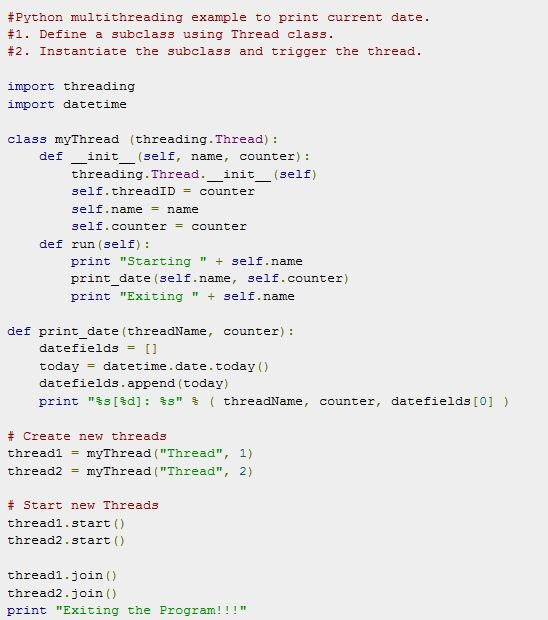
\includegraphics[width=0.75\textwidth]{figures/Thread}}
	\caption{Mengimplementasikan Thread menggunakan Threading}
	\label{Mengimplementasikan Thread menggunakan Threading}
\end{figure}

\chapter{XML Processing}
% Kelas D4 TI 3B Kelompok 3
% Diana Satima Gistivani 1154018
% M. Amran Hakim Siregar 1154106
% Indah Rahmawati 1154070
% Rizky Abdul Ghani Suherli 1154058


\section{Python XML Processing}
  XML adalah bahasa open source portable yang mungkinkan pemrogram mengemangkan aplikasi yang dapat dibaca oleh aplikasi lain, bahasa markup untuk keperluan umum yang disarankan oleh W3C untuk membuat dokumen markup keperluan pertukaran data antar sistem yang beraneka ragam. XML merupakan kelanjutan dari HTML (HyperText Markup Language) yang merupakan bahasa standar untuk melacak Internet.
terlepas dari sistem operasi dan bahasa pengembangnya .
\subsection{Apa itu XML}
  Extensible Markup Languange (XML) adalah bahasa markup seperti HTML atau SGML. 
Ini direkomendasikan oleh World Wide Web Consortium dan tersedia sebagai standar terbuka.
XML sangat berguna untuk mencatat data berukuran kecil dan menengah tanpa memerlukan tulang punggung berbasis SQL  
Pada kenyataanya dalam dunia komputer, sistem komputer dan database mengandung data yang tidak kompatibel satu sama lain. Dengan demikian tidak mungkin terjadinya pertukaran data melalui internet jika terdapat perbedaan sistem operasi dan aplikasi database yang digunakan.
Dengan menggunakan XML untuk pertukaran data, masalah perbedaan platform dan aplikasi tidak perlu diresahkan lagi. karena data yang disimpan pada XML dapat dibaca oleh berbagai macam platform dan aplikasi.

\subsection{Keunggulan dan Kelemahan Python XML Processing}
\subsubsection{Keunggulan Python XML Processing}
\begin{enumerate}
Keunggulan dari python dapat dijabarkan dari faktor-faktor berikut ini :
\item Quality : Python merupakan piranti lunak yang memakai meodologi reusability sehingga komponen-komponen pembangun piranti      lunak mudah digunakan dan diatur.
\item Productivity : penulisan program menggunakan python lebih mudah, karena interpreter menangani source code secara terpisah pada lower-level language.Interpreter menangani tipe deklarasi variabel,manajemen memory dan source code.
\item Portability : program python dapat dieksekusi di berbagai jenis komputer.Dengan demikian proses eksekusi program dapat dilakukan tanpa mengubah source code program.
\item Integration : phyton dirancang untuk dapat berinteraksi dengan aplikasi lain.Dengan demikian,program yang dibangun dengan bahasa pemrograman lain dapat dieksekusi dengan mudah padascript phyton dengan menggunakan function bahasa pemrograman lainnya.
\item Tidak ada tahapan kompilasi dan penyambungan (link) sehingga kecepatan perubahan pada masa pembuatan sistem aplikasi meningkat.
\item Tidak ada deklarasi tipe data yang merumitkan sehingga program menjadi lebih sederhana, singkat, dan fleksible.
\item Manajemen memori otomatis yaitu kumpulan sampah memori sehingga dapat menghindari pencacatan kode.
\item Tipe data dan operasi tingkat tinggi yaitu kecepatan pembuatan sistem aplikasi menggunakan tipe objek yang telah ada.
\item Pemrograman berorientasi objek.
\item Pelekatan dan perluasan dalam C.
\item Terdapat kelas, modul, eksepsi sehingga terdapat dukungan pemrograman skala besar secara modular.
\item Pemuatan dinamis modul C sehingga ekstensi menjadi sederhana dan berkas biner yang kecil
\item Pemuatan kembali secara dinamis modul phyton seperti memodifikasi aplikasi tanpa menghentikannya.
\item Model objek universal kelas Satu.
\item Konstruksi pada saat aplikasi berjalan.
\item Interaktif, dinamis dan alamiah.
\item Akses hingga informasi interpreter.
\item Portabilitas secara luas seperti pemrograman antar platform tanpa ports.
\item Kompilasi untuk portable kode byte sehingga kecepatan eksekusi bertambah dan melindungi kode sumber.
\item Antarmuka terpasang untuk pelayanan keluar seperti perangkat Bantu system, GUI, persistence, database, dll.


\end{enumerate}
 
\subsection {Arsitektur XML dan API}
  Perpustakaan standar Python menyediakan seperangkat antarmuka minimal tapi berguna untuk bekerja dengan XML. Dua API yang paling dasar dan umum digunakan untuk data XML adalah antarmuka SAX dan DOM. 
\subsubsection {System Arsitektur XML}
\begin{enumerate}
Sistem terdiri dari 3 lapisan yaitu :
\item lapisan database :Lapisan ini digunakan untuk menyimpan dokumen XML.Dalam system ini digunakan DBMS SQL Server.SQL
Server mengenalkan tipe data XML.Tipe data ini dapat digunakan dalam definisi tabel untuk mendefinisikan tipe sebuah kolom, tipe variabel dalam kode prosedural Transact-SQL, dan sebagai parameter prosedur.
\item lapisan bahasa query : XML, seperti basisdata relasional, mempunyai bahasa query sendiri yang dioptimasi untuk format data.Berpasangan dengan tipe data xml, hal ini mempercepat dan mengefisienkan penyimpanan dan temukembali data XML.
\item lapisan aplikasi : Lapisan ini merupakan antarmuka menggunakan bahasa Indonesia. Bahasa pemrograman yang digunakan adalah Java.Java menyediakan banyak fasilitas yang memudahkan untuk mengimplementasikan system yang dibuat.

\subsubsection {SAX}
  API sederhana untuk XML (SAX): mendaftarkan panggilan kemali untuk acara yang diminati dan kemudian membiarkan parser berjalan melalui dokumen. Ini berguna bila dokumen berukuran besar atau memiliki keterbatasan memori, ini memparsing file tidak pernah tersimpan dalam memori. Biasanya juga SAX ini dapat di pakai oleh Generator untuk membaca file XML dan pesan SAX ini juga biasa disebut dengan istilah event. SAX akan di kirimkan oleh Generator ke pipeline. SAX atau event ini juga dapat mengirimkan sebuah dokumen atau lampiran yang artinya SAX atau event ini dapat di proses nantinya.
  
\subsubsection {DOM}
  API Document Objek Model (DOM): ini adalah rekomendasi World Wide Web Consortium dimana keseluruhan file dibaca ke memori dan disimpan dalam bentuk hierarkies (tree-based) untuk mewakili semua fitur dokumen XML. 

SAX jelas tidak bisa memproses informasi secepat DOM saat bisa bekerjadengan file besar. Di sisi lain, menggunakan DOM secara eklusifenar-benar dapat membunuh sumber daya, terutama jika digunakan pada banyak file kecil. SAX hanya bisa dibaca sementara DOM mengizinkan perubahan pada file XML. Kedua API yang berbeda ini saling melengkapi satu sama lain, tidak ada alasan mengapa tidak dapat menggunakannya untuk proyek besar. 

Contoh: 
\begin{verbatim}
<collection shelf="New Arrivals"> 
<movie title="Enemy Behind"> 
  <type>War, Thriller</type> 
  <format>DVD</format> 
  <year>2003</year> 
  <rating>PG</rating> 
  <stars>10</stars>
  <description>Talk about a US-Japan war</description> 
</movie> 
<movie title="Transformers"> 
  <type>Anime, Science Fiction</type> 
  <format>DVD</format> 
  <year>1989</year> 
  <rating>R</rating> 
  <stars>8</stars> 
  <description>A schientific fiction</description> 
</movie> 
  <movie title="Trigun"> 
  <type>Anime, Action</type> 
  <format>DVD</format> 
  <episodes>4</episodes>  
  <rating>PG</rating> 
  <stars>10</stars> 
  <description>Vash the Stampede!</description> 
</movie>
<movie title="Ishtar"> 
  <type>Comedy</type> 
  <format>VHS</format> 
  <rating>PG</rating> 
  <stars>2</stars> 
  <description>Viewable boredom</description> 
</movie> 
</collection> 
\end{verbatim}


\subsection{Parsing XML dengan API SAX}
  SAX adalah antarmuka standar untuk parsing XML berbasis event. Parsing XML dengan SAX umumnya mengharuskan untuk membuat dengan subclassing xml.sax.
  ControlHandler menangani tag dan atribut tertentu dari XML. Objek ControlHandler menyediakan metode untuk menangani berbagai aktivitas parsing. Parsing memanggil metode ControlHandler saat memparsing file XML.
  Metode startDocument dan endDocument disebut awal dan akhir setiap elemen. Jika parsing tidak dalam mode namespace, metode startElement (tag attribute) dan endElement (tag) dipanggil. Jika tidak, metode yang sesuai startElemenNS dan endElemenNS dipanggil. 

Berikut ini metode penting untuk memahami sebelum melanjutkan ke materi berikutnya : 
\begin{enumerate}
  \item Metode berikut membuat objek parsing baru dan mengembalikannya. Objek parsing diuat akan menjadi tipe parsing pertama yang ditemukan sistem.
  \item xml.sax.make parser([parser list])
\end{enumerate}

Berikut adalah detail parameternya : 
\begin{enumerate}
  \item Parser list : pilihan argumen yang terdiri dari daftar parsing untuk digunakan yang semuanya harus menerapkan metode {make    parse}.
  \item Metode berikut membuat parsing SAX dan menggunakannya untuk mengurai dokumen. xml.sax.parser(xmlfile, contenthandler[, errorhandler])
\end{enumerate}

Membuat parsing SAX dan mengurai string XML yang ditentukan : 
xml.sax.parsertring(xmlstring,contenthandler[, errorhandler])

Brikut ini adalah detail nama dari parameter : 
\begin{enumerate}
  \item  {XMLstring}  = Nama dari string yang bisa dibaca.
  \item  {ContentHandler} = Menjadi objek ContenHandler.
  \item  {ErrorHandler} = Menjadi objek ErorHandler SAX. 
\end{enumerate}

Contoh : 
\begin{verbatim}
  \#  
  /usr/bin/python
import xml.sax 
class MovieHandler( xml.sax.ContentHandler ): 
~~ def init (self): 
~~~~~ self.CurrentData = "" 
~~~~~ self.type = "" 
~~~~~ self.format = "" 
~~~~~ self.year = "" 
~~~~~ self.rating = "" 
~~~~~ self.stars = "" 
~~~~~ self.description = "" 
~~ \#  Call when an element starts 
~~ def startElement(self, tag, attributes):
~~~~~ self.CurrentData = tag 
~~~~~ if tag == "movie": 
~~~~~~~~ print "*****Movie*****" 
~~~~~~~~ title = attributes["title"] 
~~~~~~~~ print "Title:", title 
~~ \#  Call when an elements ends 
~~ def endElement(self, tag): 
~~~~~ if self.CurrentData == "type":
~~~~~~~~ print "Type:", self.type 
~~~~~ elif self.CurrentData == "format": 
~~~~~~~~ print "Format:", self.format 
~~~~~ elif self.CurrentData == "year": 
~~~~~~~~ print "Year:", self.year 
~~~~~ elif self.CurrentData == "rating": 
~~~~~~~~ print "Rating:", self.rating 
~~~~~ elif self.CurrentData == "stars": 
~~~~~~~~ print "Stars:", self.stars 
~~~~~ elif self.CurrentData == "description": 
~~~~~~~~ print "Description:", self.description 
~~~~~ self.CurrentData = "" 
~~ \#  Call when a character is read 
~~ def characters(self, content): 
~~~~~ if self.CurrentData == "type":
~~~~~~~~ self.type = content 
~~~~~ elif self.CurrentData == "format": 
~~~~~~~~ self.format = content 
~~~~~ elif self.CurrentData == "year": 
~~~~~~~~ self.year = content 
~~~~~ elif self.CurrentData == "rating": 
~~~~~~~~ self.rating = content 
~~~~~ elif self.CurrentData == "stars":
~~~~~~~~ self.stars = content 
~~~~~ elif self.CurrentData == "description": 
~~~~~~~~ self.description = content 
if (name  == " main "): 
~~ \#  create an XMLReader 
~~ parser = xml.sax.make parser() 
~~ \#  turn off namepsaces
~~ parser.setFeature(xml.sax.handler.feature namespaces, 0) 
~~ \#  override the default ContextHandler 
~~ Handler = MovieHandler() 
~~ parser.setContentHandler( Handler )
~~ parser.parse("movies.xml") 
\end{verbatim}

Ini akan menghasilkan hasil sebagai berikut: 
\begin{verbatim}
{*****Movie******} 
{*****Movie*****} 
{Title: Enemy Behind} 
{Type: War, Thriller} 
{Format: DVD} 
{Year: 2003} 
{Rating: PG} 
{Stars: 10} 
{Description: Talk about a US-Japan war}
{*****Movie*****} 
{Title: Transformers} 
{Type: Anime, Science Fiction}
{Format: DVD} 
{Year: 1989} 
{Rating: R}
{Stars: 8} 
{Description: A schientific fiction} 
{*****Movie*****} 
{Title: Trigun} 
{Type: Anime, Action} 
{Format: DVD}
{Rating: PG} 
{Stars: 10} 
{Description: Vash the Stampede!} 
{*****Movie*****} 
{Title: Ishtar}
{Type: Comedy} 
{Format: VHS}
{Rating: PG} 
{Stars: 2} 
\end{verbatim}

\subsection{2.3 Parsing XML dengan API DOM} 
Document Ovject Model (DOM) adalah API lintas bahasa dari World Wide Web Consortium (W3C) untuk mengakses dan memodifikasi dokumen XML.  DOM sangat berguna untuk aplikasi akses acak. SAX hanya memungkinkan melihat satu bit dokumen sekaligus. Jika melihat satu elemen SAX, tidak memiliki akses ke yang lain. Berikut adalah cara termudah untuk memuat dokumen XML dengan cepat dan membuat objek minidom menggunakan modul xml.dom. Objek minidom menyediakan metode parsing sederhana yang dengan cepat memuat pohon DOM dari file XML. \par
Contoh~frase memanggil fungsi  parsing (file [,parsing]) dari objek minidokumen untuk mengurai file XML yang ditunjuk oleh file ke objek pohon DOM.
\begin{enumerate}
\item $  \#  $!/usr/bin/python
from xml.dom.minidom import parse 
import xml.dom.minidom 
\item $  \#  $ Open XML document using minidom parser
DOMTree = xml.dom.minidom.parse("movies.xml") 
collection = DOMTree.documentElement 
if collection.hasAttribute("shelf"): 
print "Root element :  $  \%  $s"  $  \%  $ collection.getAttribute("shelf") 
\item $  \#  $ Get all the movies in the collection 
movies = collection.getElementsByTagName("movie") 
\item $  \#  $ Print detail of each movie. 
for movie in movies: 
print "*****Movie*****" 
if movie.hasAttribute("title"): 
print "Title:  $  \%  $s"  $  \%  $ movie.getAttribute("title") 
type = movie.getElementsByTagName('type')[0] 
print "Type:  $  \%  $s"  $  \%  $ type.childNodes[0].data 
format = movie.getElementsByTagName('format')[0] 
print "Format:  $  \%  $s"  $  \%  $ format.childNodes[0].data 
rating = movie.getElementsByTagName('rating')[0] 
print "Rating:  $  \%  $s"  $  \%  $ rating.childNodes[0].data 
description = movie.getElementsByTagName('description')[0] 
print "Description:  $  \%  $s"  $  \%  $ description.childNodes[0].data 
Ini akan menghasilkan hasil sebagai berikut : 
Root element : New Arrivals 
*****Movie***** 
Title: Enemy Behind 
Type: War, Thriller 
Format: DVD 
Rating: PG 
Description: Talk about a US-Japan war 
*****Movie***** 
Title: Transformers 
Type: Anime, Science Fiction 
Format: DVD 
Rating: R 
Description: A schientific fiction 
*****Movie***** 
Title: Trigun 
Type: Anime, Action 
Format: DVD 
Rating: PG 
Description: Vash the Stampede! 
*****Movie***** 
Title: Ishtar 
Type: Comedy 
Format: VHS 
Rating: PG
Description: Viewable boredom 
\end{enumerate}

\subsection{Membangun Parsing Document XML menggunakan Python} 
Python mendukung untuk bekerja dengan berbagai bentuk markup data terstruktur. Selain mengurai xml.etree. \textit{ElementTree} mendukung pembuatan dokumen XML yang terbentuk dengan baik dari objek elemen yang dibangun dalam aplikasi. Kelas elemen digunakakan saat sebuah dokumen diurai untuk mengetahui bagaimana menghasilkan bentuk serial dari isinya kemudian dapat ditulis ke sebuah file.  
Untuk membuat instance elemeb gunakan fungsi elemen contructor dan \textit{SubElemen()} pabrik. 
Import xml.etree.ElementTree as xml \par
\vspace{12pt}
\noindent 
{\fontsize{10pt}{10pt}\selectfont filename =  $ " $/home/abc/Desktop/test $  \_  $xml.xml $ " $} \par
\noindent 
{\fontsize{10pt}{10pt}\selectfont toot = xml.Element( $ " $Users $ " $)} \par
\noindent 
{\fontsize{10pt}{10pt}\selectfont userelement = xml.Element( $ " $user $ " $)} \par
\noindent 
{\fontsize{10pt}{10pt}\selectfont root.append(userelement)} \par
\noindent 
\vspace{10pt}
\noindent 
Bila menjalankan ini, akan menghasilkan sebagai berikut : \par
\noindent 
{\fontsize{10pt}{10pt}\selectfont <Users>} \par
\noindent 
{\fontsize{10pt}{10pt}\selectfont  \hspace*{0.5in} <user>} \par
\noindent 
{\fontsize{10pt}{10pt}\selectfont  \hspace*{0.5in} <user>} \par
\noindent 
{\fontsize{10pt}{10pt}\selectfont </Users>} \par
\vspace{10pt}
\vspace{10pt}
\vspace{10pt}
\noindent 
Tambahkan anak-anak pegguna \par
\vspace{10pt}
\noindent 
{\fontsize{10pt}{10pt}\selectfont Uid = xml.SubElement(userelement,  $ " $uid $ " $)} \par
\noindent 
{\fontsize{10pt}{10pt}\selectfont Uid.text =  $ " $1 $ " $} \par
\vspace{10pt}
\noindent 
{\fontsize{10pt}{10pt}\selectfont FirstName = xml.SubElement(userelement,  $ " $FirstName $ " $)} \par
\noindent 
{\fontsize{10pt}{10pt}\selectfont FirstName.text =  $ " $testuser $ " $} \par
\vspace{10pt}
\noindent 
{\fontsize{10pt}{10pt}\selectfont LastName = xml.SubElement(userelement,  $ " $LastName $ " $} \par
\noindent 
{\fontsize{10pt}{10pt}\selectfont LastName.text =  $ " $testuser $ " $} \par
\vspace{10pt}
\noindent 
{\fontsize{10pt}{10pt}\selectfont Email = xml.SubElement(userelement,  $ " $Email $ " $)} \par
\noindent 
{\fontsize{10pt}{10pt}\selectfont Email.text = {mailto:testuser@test.com}{testuser@test.com}
} \par
\vspace{10pt}
\noindent 
{\fontsize{10pt}{10pt}\selectfont state = xml.SubElement(userelemet,  $ " $state $ " $)} \par
\noindent 
{\fontsize{10pt}{10pt}\selectfont state.text =  $ " $xyz $ " $} \par
\vspace{10pt}
\noindent 
{\fontsize{10pt}{10pt}\selectfont location = xml.SubElement(userelement,  $ " $location)} \par
\noindent 
{\fontsize{10pt}{10pt}\selectfont location.text = abc} \par
\vspace{10pt}
\noindent 
{\fontsize{10pt}{10pt}\selectfont tree = xml.ElementTree(root)} \par
\noindent 
{\fontsize{10pt}{10pt}\selectfont with open(filename,  $ " $w $ " $) as fh:} \par
\noindent 
{\fontsize{10pt}{10pt}\selectfont tree.write(fh)} \par
\vspace{10pt}
\noindent 
 \hspace*{0.5in} Pertama buat elemen root dengan mengunakan fungsi \textit{ElementTree}. Kemudian membuat elemen pegguna dan menambahkannya ke root. Selanjutnya membuat \textit{SubElement }dengan melewatkan elemen pengguna (userelement) ke \textit{SubElemen} beserta namanya seperto  $ " $FirstName $ " $. Kemudian untuk setiap \textit{SubElement} tetapkan properti teks untuk memberi nilai. Di akhir, membuat \textit{ElementTree} dan menggunakannya untuk menulis XML ke file. \par
\noindent 
 \hspace*{0.5in} Jika menjalankan ini akan menjadi sebagai berikut : \par
\noindent 
 {\fontsize{10pt}{10pt}\selectfont <users>} \par
\noindent 
{\fontsize{10pt}{10pt}\selectfont  \hspace*{0.5in} <user>} \par
\noindent 
{\fontsize{10pt}{10pt}\selectfont  \hspace*{0.5in}  \hspace*{0.5in} <uid>1</uid>} \par
\noindent 
{\fontsize{10pt}{10pt}\selectfont  \hspace*{0.5in}  \hspace*{0.5in} <FirstName>testuser</FirstName>} \par
\noindent 
{\fontsize{10pt}{10pt}\selectfont  \hspace*{0.5in}  \hspace*{0.5in} <LastName>testuser</LastName>} \par
\noindent 
{\fontsize{10pt}{10pt}\selectfont  \hspace*{0.5in}  \hspace*{0.5in} <state>xyz</state>} \par
\noindent 
{\fontsize{10pt}{10pt}\selectfont  \hspace*{0.5in}  \hspace*{0.5in} <location>abc</location>} \par
\noindent 
{\fontsize{10pt}{10pt}\selectfont  \hspace*{0.5in} </user>} \par
\noindent 
{\fontsize{10pt}{10pt}\selectfont </Users>} \par
\vspace{10pt}
\noindent 
Parsing XML Documen : \par
\vspace{12pt}
\noindent 
{\fontsize{10pt}{10pt}\selectfont import xml.etree.ElementTree as ET} \par
\noindent 
{\fontsize{10pt}{10pt}\selectfont tree = ET.parse(‘Your $  \_  $XML $  \_  $file $  \_  $path’)} \par
\noindent 
{\fontsize{10pt}{10pt}\selectfont root = tree.getroot()} \par
\noindent 
{\fontsize{10pt}{10pt}\selectfont 

 %%%%%%%%%%%%  Start New Page here %%%%%%%%%%%%%%


\newpage

}\vspace{10pt}
\vspace{10pt}
\noindent 
Disini \textit{getroot()} akan mengembalikan elemen dari dokumen XML \par
\vspace{10pt}
\noindent 
{\fontsize{10pt}{10pt}\selectfont <Users version= $ " $1.0 $ " $ languange= $ " $SPA $ " $>} \par
\noindent 
{\fontsize{10pt}{10pt}\selectfont  \hspace*{0.5in} <user>} \par
\noindent 
{\fontsize{10pt}{10pt}\selectfont  \hspace*{0.5in}  \hspace*{0.5in} <uid>1</uid>} \par
\noindent 
{\fontsize{10pt}{10pt}\selectfont  \hspace*{0.5in}  \hspace*{0.5in} <FirstName>testuser</FirstName>} \par
\noindent 
{\fontsize{10pt}{10pt}\selectfont  \hspace*{0.5in}  \hspace*{0.5in} <LastName>testuser</LastName>} \par
\noindent 
{\fontsize{10pt}{10pt}\selectfont  \hspace*{0.5in}  \hspace*{0.5in} <Email>testuser@tes.com/Email>} \par
\noindent 
{\fontsize{10pt}{10pt}\selectfont  \hspace*{0.5in}  \hspace*{0.5in} <state>xyz</state>} \par
\noindent 
{\fontsize{10pt}{10pt}\selectfont  \hspace*{0.5in}  \hspace*{0.5in} <location>abc</location>} \par
\noindent 
{\fontsize{10pt}{10pt}\selectfont  \hspace*{0.5in} </user>} \par
\noindent 
{\fontsize{10pt}{10pt}\selectfont </Users>} \par
\vspace{12pt}


\chapter{GUI Programming}
\documentclass [12pt,a4paper,notitlepage,oneside,bahasa]{article}
\usepackage[left=3.00 cm, right=2.00 cm, bottom=2.00 cm, top=3.00 cm]{geometry}
\begin{document}
\title{\textbf GUI Programming}
\maketitle

Python menyediakan berbagai pilihan untuk mengembangkan antarmuka pengguna grafis (GUIs). 
Berikut dibawah ini merupakan berbagai pilihan yang disediakan oleh Python :
\begin{itemize}
\item Tkinter \par
Tkinter merupakan standar bahasa python yang ditetapkan untuk membangun suatu antarmuka pengguna grafik (GUI). 
\item wxPython \par
wxPython adalah toolkit antarmuka pengguna grafis (GUI) yang digunakan dalam skripsi ini dan ini adalah pembungkus untuk toolkit wxWidgets.
\item Jpython \par
Port Python untuk java yang memberikan Python script akses tanpa batas ke perpustakaan kelas java pada mesin lokal \par
\end{itemize}
\vspace{12pt}
\noindent 
\section{\textbf Tkinter Pemrograman}
Tkinter adalah perpustakaan GUI standar untuk Python. Python bila dikombinasikan dengan Tkinter menyediakan cara yang amat mudah dan cepat untuk membuat aplikasi GUI. Tkinter menyediakan antarmuka yang berorientasi objek yang kuat untuk toolkit Tk GUI.
 \hspace*{0.5in} Membuat aplikasi GUI menggunakan Tkinter adalah tugas yang mudah. Yang diperlukan adalah melakukan langkah-langkah sebagai berikut : 
\begin{enumerate} 
	\item Mengimpor Tkinter modul 
	\item Buat jendela utama aplikasi GUI
	\item Tambahkan satu atau lebih dari widget tersebut diatas ke aplikasi GUI
	\item Masukkan acara loop utama untuk mengambil tindakan terhadap setiap peristiwa dipicu oleh pengguna
\end{enumerate}

 %%%%%%%%%%%%  Start New Page here %%%%%%%%%%%%%%


\newpage

\vspace{12pt}
\vspace{12pt}
\noindent 
Contoh : 
\begin{verbatim}
#!/usr/bin/python 
import Tkinter 
top = Tkinter.Tk()
# Code to add widgets will go here...
top.mainloop()
\end{verbatim}

\section{\textbf Tkinter Widget} \par
\noindent 
 \hspace*{0.5in} Tkinter menyediakan berbagai kontrol seperti tombol, label dan kotak teks yang digunakan dalam aplikasi GUI. 
 Kontrol ini biasanya disebut widget.
\noindent 
 \hspace*{0.5in} Saat ini ada 15 jenis widget di Tkinter. berikut adalah contoh widget serta penjelasan singkat pada tabel ini:


 %%%%%%%%%%%%  Table No:1 Here %%%%%%%%%%%%%%


\begin{table}[h]
	\caption{Ukuran}
		\begin{center}
		\begin{tabular}{|c|c|}
			\hline
			Operator & Penjelasan \\
			\hline
			Button & Menampilkan tombol dalam aplikasi\\
			Canvas & Menggambar bentuk seperti garis, oval, poligon dan persegi panjang dalam aplikasi\\
			Checkbutton & Menampilkan sejumlah pilihan sebagai kotak centang. Pengguna dapat memilih beberapa pilihan pada suatu waktu
			Entry & Menampilkan bidang garis teks tunggal untuk menerima nilai-nilai dari pengguna\\
			Frame & Wadah untuk mengatur widget lainnya\\
			Label & Memberikan keterangan garis single untuk widget lainnya. Hal ini berisi gambar\\
			Listbox & Menyediakan daftar pilihan kepada pengguna\\
			Menubutton & Menampilkan menu dalam aplikasi\\
			Menu & Memberikan berbagai perintah untuk pengguna. Perintah-perintah ini terkandung di dalam MenuButton\\
			Message & Menampilkan bidang teks multiline untuk menerima nilai-nilai dari pengguna\\
			RadioButton & Menampilkan sejumah pilihan sebagai tombol radio. Pengguna dapat memilih hanya satu pilihan pada suatu waktu\\
			Scale & Menyediakan widget slide\\
			Scrollbar & Menambah kemampuan bergulir ke berbagai widget seperti kotak daftar\\
			Text & Menampilka teks dalam beberapa garis\\
			Toplevel & Menyediakan wajah jendela terpisah\\
			PanedWindow & Wadah yang mengandung sejumlah panel disusun horizontal atau vertikal\\
			LabelFrame & Wadah widget sederhana. Bertindak sebagai spacer atau wajah untuk layout jendela kompleks\\
			TkMessageBox & Menampilkan kotak pesan dalam aplikasi\\
			Spinbox & Memilih sejumlah tetap nilai-nilai&\\
		\hline
		\end{tabular}
		\end{center}
	\begin{tablenotes}
	\end{tablenotes}
\end{table}

	


 %%%%%%%%%%%%  Table No:1 Ends Here %%%%%%%%%%%%%%


\vspace{12pt}
subsection{Atribut Tkinter}
\noindent 
 \hspace*{0.5in} Beberapa atribut umum sebagai ukuran, warna dan font ditentukan. Berikut adalah beberapa atribut standar :
\noindent 
\begin{enumerate}
\item Ukuran 
Berbagai panjang, lebar, dan dimensi lain dari widget digambarkan dalam banyak unit yang berbeda seperti 
\item Jika menetapkan dimensi ke integer diasumsikan dalam piksel 
\item Menentukan unit dengan menentukan dimensi untuk string yang berisi sejumlah diikuti oleh :
\end{itemize}
 


 %%%%%%%%%%%%  Table No:2 Here %%%%%%%%%%%%%%


\begin{table}[ht]
	\caption{Ukuran}
	\bein{center}
	\begin{tabular}{|c|c|}
		\hline
		Karakter&  Penjelasan \cr
		\hline
		c&Sentimeter\\
		i&Inci\\
		m&Milimeter\\
		p&Poin printer\\
		\hline
	\end{tabular}
	\end{center}
	\begin{tablenotes}
	\end{tablenotes}
\end{table}


 %%%%%%%%%%%%  Table No:2 Ends Here %%%%%%%%%%%%%%

 
 \hspace*{0.5in} \vspace{12pt}
 subsection{Panjang Tkinter}
 \hspace*{0.5in} Tkinter mengungkapkan panjang sebagai integer jumlah piksel. Berikut ini adalah daftar pilihan panjang umum:
\noindent 
\begin{itemize}
	\item borderwidth
	Lebar batas yang memberikan tampilan tiga dimensi untuk widget
	\item highlightthickness
	Lebar puncak persegi panjang ketika widget memiliki fokus
 	\item padX padY
	Ruang tambahan widget dari manajer tata letak luar minimum widget perlu menampilkan isinya di x dan y arah
	\item selectborderwidth
	Lebar perbatasan tiga dimensi disekitar dipilih item widget
	\item wraplength \par
	Panjang garis maksimum untuk widget yang melakukan kata membungkus
	\item height
	Tinggi diinginkan widget
	\item underline
	Indeks karakter untuk menggarisawahi dalam teks widget 
	\item width
	\item Lebar diinginkan widget
\end{itemize}
 
\noindent 
subsection{Warna Tkinter}
\noindent 
Tkinter memiliki warna dengan string. Ada dua cara umum untuk menentukan sebuah warna di Tkiter, yaitu : \par
\noindent 
\begin{itemize}
	\item Menggunakan string menentukan proporsi merah, hijau dan biru didigit heksadesimal. Misalnya  `` \#ffff '' putih,  ``  \#000000 '' hitam dan  ``\#000fff000 '' hijau.
\noindent 
	\item Menggunakan lokal standar nama warna . warna-warna ``white'', ``black'',  ``green'' dan  ``magenta'' akan selalu tersedia.
\end{itemize}

\vspace{12pt}
Pilihan warna umum :
\noindent 
\begin{itemize}
	\item activebackground \par
	Warna latar berlakang untuk widget ketika widget aktif \par
	\noindent 
	\item activeforeground \par
	Warna depan untuk widget ketika widget aktif \par
	\noindent 
	\item background \par
	Merepresentasikan sebagai \textit{bg} \par
	\noindent 
	\item disableforeground \par
	Warna depan untuk widget ketika widget dinonaktifkan \par
	\noindent 
	\item foreground \par
	Merepresentasikan fg \par
	\noindent 
	\item highlightbackground \par
	Warna latar belakang dari daerah puncak ketika widget memiliki fokus \par
	\noindent 
	\item hightlightcolor \par
	Warna depan dari wilayah puncak ketika widget memiliki fokus \par
	\noindent 
	\item selectbackground \par
	Warna latar belakang untuk item yang dipilih dari widget \par
	\noindent 
	\item selectforeground \par
	Warna depan untuk item yang dipilih dari widget \par
	\noindent 
	\item Font \par
	\noindent 
	Sebagai tupel yang elemen pertama adalah keluarga font diikuti dengan string yang berisi satu atau lebih gaya pengubah tebal,miring, garis bawah dan overstrike. 
	end{itemize}
	\noindent 
Contoh : \par
	\begin{itemize}
		\noindent
		\item ( ``Helvetica'', ``16 '') untuk 16 \- point Helvetica biasa \par
		\noindent 
		\item ( ``Times'', ``24 '',``beranimiring'') untuk 24 \- point kali miring tebal
	\end{itemize}
 		\par
\vspace{12pt}
Dapat membuat  ``font object'' dengan mengimpor modul tkFont dan menggunakan kelas konstruktor font nya : \par
Import tkFont \par
Font = tkFont.Font (option, ....) \par
\vspace{12pt}
Berikut adalah daftar pilihan : \par
\noindent 
\begin{itemize}
	\item Family \par
	Font nama keluarga sebagai string \par
	\noindent 
	\item Size \par
	Font tinggi sebagai integer dalam poin \par
	\noindent 
	\item Weight \par
	Bold untuk teal, normal untuk berat badan secara teratur \par
	\noindent 
	\item Slant \par
	Italic untuk miring, roman untuk unstlanted \par
	\noindent 
	\item Underline \par
	1 untuk teks yang digarisbawahi, 0 untuk normal \par
	\noindent 
	\item Overstrike \par
	1 untuk teks telak, 0 untuk normal \par
	Jika berjalan di bawah X window system, dapat menggunakan salah satu nama font X. Sebagai contoh, font bernama  \verb|"-*lucidatypewriter-medium-r-*-*-*-140-*-*-*"| adalah favorit fixed-width font penulis untuk digunakan pada layar. \par
	\noindent 
	\item Jangkar \par
	\noindent 
	Jangkar digunakan untuk mendefinisikan mana teks diposisikan relatif terhadap titik acuan. Berikut adalah daftar kemungkinan konstanta yang dapat digunakan :
	\noindent
	\begin{itemize}
		\item NW  
		\item N
		\item NE
		\item W
		\item TENGAH
		\item E
		\item SW
		\item S
		\item SE
	\end{itemize}
\end{itemize}
 \par
\vspace{12pt}
Jika menggunakan tengah sebagai jangkar tek, tek akan ditengahkan horizontal dan vertikal disekitar titik referensi. \par
Jangkar NW akan posisi teks sehingga titik referensi bertepatan dengan laut sudut kotak berisi teks \par
Jangakr W akan pusat teks secara vertikal disekitar satu titik referensi dengan tepi kiri kotak teks yang melewati titik itu dan sebagainya. \par
Jika membuat widget kecil didalam bingkai besar dan menggunakan jangkar = SE pilihan, widget akan ditempatkan disudut kanan bawah gambar. Jika menggunakan anchor = N sebaliknya widget akan dipusatkan disepanjang tepi atas. \par
\noindent 

subsection{Gaya relief}

Widget mengacu pada efek 3-D simulasi terbaru disekitar bagian luar widget. Berikut adalah daftar konstanta yang mungkin dapat digunakan untuk atribut:
\begin{itemize}
	\item Datar
	\item Dibesarkan
	\item Cekung
	\item Alur
	\item Punggung bukit
\end{itemize}


\vspace{12pt}
Contoh : \par
{\fontsize{10pt}{10pt}\selectfont From Tkinter import *} \par
{\fontsize{10pt}{10pt}\selectfont Import Tkinter} \par
\vspace{10pt}
{\fontsize{10pt}{10pt}\selectfont top = Tkinter.Tk()} \par
{\fontsize{10pt}{10pt}\selectfont B1 = Tkinter.Button(top, text= $ " $FLAT $ " $, relief=FLAT)} \par
{\fontsize{10pt}{10pt}\selectfont B2 = Tkinter.Button(top, text= $ " $RAISED $ " $, relief=RAISED)} \par
{\fontsize{10pt}{10pt}\selectfont B3 =Tkinter.Button(top, text= $ " $SUNKEN $ " $, relief=SUNKEN)} \par
{\fontsize{10pt}{10pt}\selectfont B4=Tkinter.Button(top, text= $ " $GROOVE $ " $, relief=GROOVE)} \par
{\fontsize{10pt}{10pt}\selectfont B5=Tkinter.Button(top, text= $ " $RIDGE $ " $, relief=RIDGE)} \par
\vspace{10pt}
{\fontsize{10pt}{10pt}\selectfont B1.pack()} \par
{\fontsize{10pt}{10pt}\selectfont B2.pack()} \par
{\fontsize{10pt}{10pt}\selectfont B3.pack()} \par
{\fontsize{10pt}{10pt}\selectfont B4.pack()} \par
{\fontsize{10pt}{10pt}\selectfont B5.pack()} \par
{\fontsize{10pt}{10pt}\selectfont top.mainloop()} \par
\noindent 
Britmaps \par
\noindent 
Ada beberapa jenis bitmap yang tersedia, diantaranya: \par
\noindent 
\begin{itemize}
\item Kesalahan \par
\noindent 
\item Gray75 \par
\noindent 
\item Gray50 \par
\noindent 
\item Gray12 \par
\noindent 
\item Jam Pasir \par
\noindent 
\item Info \par
\noindent 
\item Questhead \par
\noindent 
\item Perantanyaan  \par
\noindent 
\item Peringatan\end{itemize}
 \par
\vspace{12pt}
Contoh: \par
{\fontsize{10pt}{10pt}\selectfont From Tkinter import *} \par
{\fontsize{10pt}{10pt}\selectfont Import Tkinter} \par
\vspace{10pt}
{\fontsize{10pt}{10pt}\selectfont Top = Tkinter.Tk()} \par
\vspace{10pt}
{\fontsize{10pt}{10pt}\selectfont B1 = Tkinter.Button(top, text = $ " $error $ " $, relief=RAISED,  $  \setminus  $ bitmap= $ " $error $ " $)} \par
{\fontsize{10pt}{10pt}\selectfont B2 = Tkinter.Button(top, text = $ " $hourglass $ " $, relief=RAISED,  $  \setminus  $ bitmap= $ " $hourglass $ " $)} \par
{\fontsize{10pt}{10pt}\selectfont B3 = Tkinter.Button(top, text = $ " $info $ " $, relief=RAISED,  $  \setminus  $ bitmap= $ " $info $ " $)} \par
{\fontsize{10pt}{10pt}\selectfont B4 = Tkinter.Button(top, text = $ " $question $ " $, relief=RAISED,  $  \setminus  $ bitmap= $ " $question $ " $)} \par
{\fontsize{10pt}{10pt}\selectfont B5 = Tkinter.Button(top, text = $ " $warning $ " $, relief=RAISED,  $  \setminus  $ bitmap= $ " $warning $ " $)} \par
\vspace{10pt}
{\fontsize{10pt}{10pt}\selectfont B1.pack()} \par
{\fontsize{10pt}{10pt}\selectfont B2.pack()} \par
{\fontsize{10pt}{10pt}\selectfont B3.pack()} \par
{\fontsize{10pt}{10pt}\selectfont B4.pack()} \par
{\fontsize{10pt}{10pt}\selectfont B5.pack()} \par
{\fontsize{10pt}{10pt}\selectfont top.mainloop()} \par
\noindent 
Kursor \par
\noindent 
Berikut daftar menarik : \par
\noindent 
\begin{itemize}
\item Panah \par
\noindent 
\item Lingkaran \par
\noindent 
\item Jam \par
\noindent 
\item Menyebrang \par
\noindent 
\item Dotbox \par
\noindent 
\item Bertukar \par
\noindent 
\item Fluer \par
\noindent 
\item Jantung \par
\noindent 
\item Manusia \par
\noindent 
\item Tikus \par
\noindent 
\item Bajak laut \par
\noindent 
\item Tamah \par
\noindent 
\item Antar jemput \par
\noindent 
\item Perekat \par
\noindent 
\item Laba-laba \par
\noindent 
\item Kaleng semprot \par
\noindent 
\item Bintang \par
\noindent 
\item Target \par
\noindent 
\item Tcross \par
\noindent 
\item Melakukan perjalanan \par
\noindent 
\item Menonton\end{itemize}
 \par
\vspace{12pt}
Contoh : \par
{\fontsize{10pt}{10pt}\selectfont From Tkinter import *} \par
{\fontsize{10pt}{10pt}\selectfont Import Tkinter} \par
\vspace{10pt}
{\fontsize{10pt}{10pt}\selectfont Top = Tkinter.Tk()} \par
\vspace{10pt}
{\fontsize{10pt}{10pt}\selectfont B1 = Tkinter.Button(top, text = $ " $circle $ " $, relief=RAISED,  $  \setminus  $ bitmap= $ " $circle $ " $)} \par
{\fontsize{10pt}{10pt}\selectfont B2 = Tkinter.Button(top, text = $ " $plus $ " $, relief=RAISED,  $  \setminus  $ bitmap= $ " $plus $ " $)} \par
\vspace{10pt}
{\fontsize{10pt}{10pt}\selectfont B1.pack()} \par
{\fontsize{10pt}{10pt}\selectfont B2.pack()} \par
{\fontsize{10pt}{10pt}\selectfont top.mainloop()} \par
\vspace{10pt}
\noindent 
\textbf{3.3 Manajemen Geometri} \par
\noindent 
 \hspace*{0.5in} Semua widget tkinter memiliki akses ke metode manajemen geometri tertentu, yang memiliki tujuan menggorganisir widget diseluruh wilayah widget induk. Tkinter mengekspos kelas manager geometri berikut : \par
\noindent 
\begin{itemize}
\item Metode the \textit{pack()} \par
\noindent 
Manajer geometri ini mengatur widget diblok sebelum menempatkan mereka di widget induk \par
\noindent 
\item Metode the \textit{grid()} \par
\noindent 
Manajer geometri ini mengatur widget dalam struktur tabel seperti di widget induk \par
\noindent 
\item Metode the  \textit{place()}\end{itemize} \par
\noindent 
Manajer geometri ini mengatur widget dengan menempatkan dalam posisi tertentu dalam widget induk \par
\vspace{12pt}
\noindent 
\textbf{3.4 Manfaat Tkinter} \par
Tkinter sangat sederhana. Berikut manfaat Tkinter dibandingkan GUI toolkit : \par
\noindent 
\begin{itemize}
\item 
Tkinter terdiri dari sejumlah modul.  (Tkinter)\vspace{\baselineskip}
Antarmuka Tk terletak di modul biner
bernama _tkinter (ini adalah tkinter di versi sebelumnya). Modul ini berisi lowlevel
antarmuka ke Tk, dan tidak boleh digunakan langsung oleh pemrogram aplikasi. ini
biasanya shared library (atau DLL), tapi mungkin dalam beberapa kasus secara statis terkait dengan
Penerjemah Python. \par
\noindent
\item Tkinter mudah diakses oleh siapa saja. (Accessibilty)\vspace{\baselineskip}
Tkinter merupakan toolkit yang ringan dan satu-satunya solusi GUI yang paling sederhana untuk Python sampai saat ini. Cukup menuliskan 
beberapa baris kode Python untuk membuat aplikasi GUI sederhana dengan Tkinter. Untuk menambahkan komponen baru pada Tkinter, dapat 
membuatnya dalam kode Python atau menambahkan paket ekstensi seperti Pmw, Tix, atau ttk. \par
\noindent 
\item widget root tk (widget root tk)\vspace{\baselineskip}
Untuk menginisialisasi Tkinter, kita harus membuat widget root Tk. Ini adalah jendela biasa, dengan
judul bar dan hiasan lainnya yang disediakan oleh window manager Anda. Anda seharusnya saja
buat satu widget root untuk setiap program, dan itu harus dibuat sebelum widget lainnya. \par
\noindent 
\item Tkinter mudah digunakan di semua platform (Portability)\vspace{\baselineskip}
Sebuah program Python yang dibangun menggunakan Tkinter dapat berjalan dengan baik di semua platform sistem operasi seperti Microsoft 
Windows, Linux, dan Macintosh. Dan dari segi tampilan window, akan terlihat sama dengan standar platform yang digunakan. \par
\noindent 
\item Tkinter selalu tersedia di Python (Availability)\vspace{\baselineskip}
Tkinter merupakan modul standar pada pustaka Python. Sebagian besar paket instalasi Python sudah langsung berisi Tkinter. Khusus untuk 
beberapa distro Linux, perlu menambahkan paket Tkinter secara terpisah. Pada Windows, bisa langsung menggunakan Tkinter sesaat setelah 
menginstal paket instalasi Python. \par
\noindent 
\item handles bagus di gunakan di Python (Handles)\vspace{\baselineskip}
item kandles merupakan nilai integer yang digunakan untuk mengidentifikasi item tertentu pada kanvas. Tkinter secara otomatis menugaskan 
pegangan baru ke setiap item baru yang dibuat di atas kanvas. Item Handles dapat di lewatkan ke berbagai metode kanvas baik sebagai 
bilangan bulat atau sebagai string. Tag adalah nama simbolis yang dilekatkan pada item. Tag adalah string biasa, dan bisa berisi apa 
saja kecuali spasi (asalkan tidak sesuai dengan item pegangan). \par
\noindent 
\item Modul Tkinter menyediakan kelas yang sesuai dengan berbagai jenis widget di Tk (Module)\vspace{\baselineskip}
dan sejumlah mixin dan kelas pembantu lainnya (mixin adalah kelas yang dirancang untuk menjadi
dikombinasikan dengan kelas lain menggunakan multiple inheritance). Bila Anda menggunakan Tkinter, Anda
jangan pernah mengakses kelas mixin secara langsung. \par
\noindent 
\item Dokumentasi Tkinter sangat LUAR BIASA (Documentation)\vspace{\baselineskip}
Python (plus Tkinter) ini bersifat open-source, maka banyak sekali komunitas-komunitas yng membahas Python dan Tkinter dan bisa belajar dan bertanya langsung dengan para ahli.\end{itemize}
 \par
\vspace{12pt}
\vspace{12pt}

\end{document}


\chapter{Futher Expression}


\begin{references}{3.}
\bibitem{kilby}J. S. Kilby,
``Invention of the Integrated Circuit,'' {\it IEEE Trans. Electron Devices,}
{\bf ED-23,} 648 (1976).

\bibitem{hamming}R. W. Hamming,
                 {\it Numerical Methods for Scientists and 
                 Engineers}, Chapter N-1, McGraw-Hill, 
                 New York, 1962.

\bibitem{Hu}J. Lee, K. Mayaram, and C. Hu, ``A Theoretical
               Study of Gate/Drain Offset in LDD MOSFETs''
                     {\it IEEE Electron Device Lett.,} {\bf EDL-7}(3). 152 
                     (1986).

\bibitem{beren}A. Berenbaum, 
B. W. Colbry, D.R. Ditzel, R. D Freeman, and 
K.J. O'Connor, ``A Pipelined 32b Microprocessor with 13 kb of Cache Memory,''
{it Int. Solid State Circuit Conf., Dig. Tech. Pap.,} p. 34 (1987).
\end{references}


\begin{references}{Ham62}
\bibitem[Kil76]{kilb}J. S. Kilby,
``Invention of the Integrated Circuit,'' {\it IEEE Trans. Electron Devices,}
{\bf ED-23,} 648 (1976).

\bibitem[Ham62]{hamm}R. W. Hamming,
                 {\it Numerical Methods for Scientists and 
                 Engineers}, Chapter N-1, McGraw-Hill, 
                 New York, 1962.

\bibitem[Hu86]{lee}J. Lee, K. Mayaram, and C. Hu, ``A Theoretical
               Study of Gate/Drain Offset in LDD MOSFETs''
                     {\it IEEE Electron Device Lett.,} {\bf EDL-7}(3). 152 
                     (1986).

\bibitem[Ber87]{berm}A. Berenbaum, 
B. W. Colbry, D.R. Ditzel, R. D Freeman, and 
K.J. O'Connor, ``A Pipelined 32b Microprocessor with 13 kb of Cache Memory,''
{it Int. Solid State Circuit Conf., Dig. Tech. Pap.,} p. 34 (1987).

\end{references}



%%%%%%%%%%%%%%%
%%  The default LaTeX Index
%%  Don't need to add any commands before \begin{document}
\printindex

%%%% Making an index
%% 
%% 1. Make index entries, don't leave any spaces so that they
%% will be sorted correctly.
%% 
%% \index{term}
%% \index{term!subterm}
%% \index{term!subterm!subsubterm}
%% 
%% 2. Run LaTeX several times to produce <filename>.idx
%% 
%% 3. On command line, type  makeindx <filename> which
%% will produce <filename>.ind 
%% 
%% 4. Type \printindex to make the index appear in your book.
%% 
%% 5. If you would like to edit <filename>.ind 
%% you may do so. See docs.pdf for more information.
%% 
%%%%%%%%%%%%%%%%%%%%%%%%%%%%%%

%%%%%%%%%%%%%% Making Multiple Indices %%%%%%%%%%%%%%%%
%% 1. 
%% \usepackage{multind}
%% \makeindex{book}
%% \makeindex{authors}
%% \begin{document}
%% 
%% 2.
%% % add index terms to your book, ie,
%% \index{book}{A term to go to the topic index}
%% \index{authors}{Put this author in the author index}
%% 
%% \index{book}{Cows}
%% \index{book}{Cows!Jersey}
%% \index{book}{Cows!Jersey!Brown}
%% 
%% \index{author}{Douglas Adams}
%% \index{author}{Boethius}
%% \index{author}{Mark Twain}
%% 
%% 3. On command line type 
%% makeindex topic 
%% makeindex authors
%% 
%% 4.
%% this is a Wiley command to make the indices print:
%% \multiprintindex{book}{Topic index}
%% \multiprintindex{authors}{Author index}

\end{document}

